\section{Experimental Setup}
\begin{itemize}
    \item experimental setup
    \item measurement procedure
\end{itemize}
\begin{figure}
    \centering
    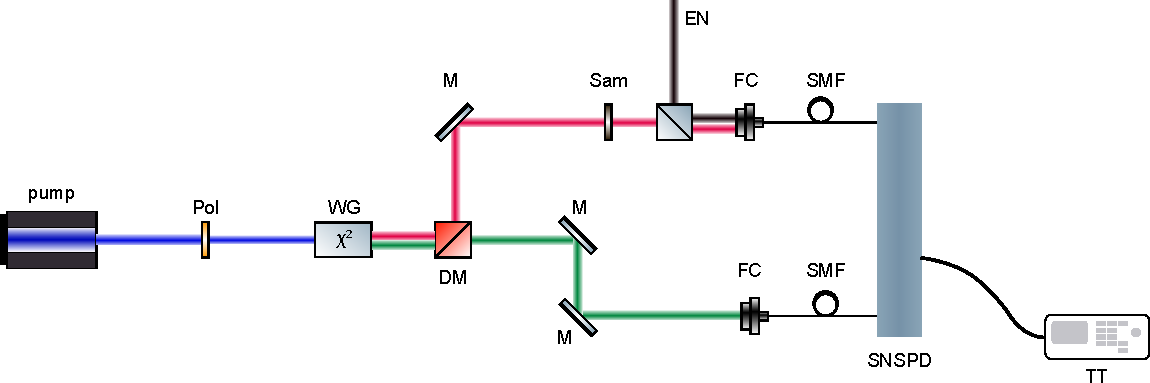
\includegraphics[width=\linewidth]{Images/bitmap.pdf}
    \caption{Caption}
    \label{fig:placeholder}
\end{figure}
\begin{figure}[!ht]
\centering
\resizebox{.9\textwidth}{!}{%
\begin{tikzpicture}
    \tikzstyle{every node}=[font=\LARGE]

    \pgfmathsetmacro{\yTop}{12.5}
    \pgfmathsetmacro{\yBottom}{8.25}
    \pgfmathsetmacro{\yMid}{\yBottom + 0.6*(\yTop - \yBottom)}
    \pgfmathsetmacro{\pLab}{\yBottom + 0.5*(\yTop - \yBottom)}
    \pgfmathsetmacro{\sLab}{\yBottom + 0.3*(\yTop - \yBottom)}
    \pgfmathsetmacro{\iLab}{\yBottom + 0.8*(\yTop - \yBottom)}
    
    
    \draw [line width=2.5pt] (3.5,8.25) -- (12.5,8.25);
    \draw [ color={rgb,255:red,0; green,0; blue,255}, line width=2pt,-{Latex[length=4mm]}] (5,8.25) -- (5,\yTop);
    \draw [line width=2.3pt, dashed] (3.75,\yTop) -- (12.5,\yTop);
    \draw [ color={rgb,255:red,255; green,0; blue,0}, line width=1pt,-{Latex[length=4mm]}] (10,\yTop) -- (10,\yMid);
    \draw [ color={rgb,255:red,0; green,255; blue,0}, line width=1pt,-{Latex[length=4mm]}] (10,\yMid) -- (10,8.25);
    \node [font=\LARGE, color={rgb,255:red,0; green,0; blue,255}] at (4.25,\pLab) {$\omega_{\text{P}}$};
    \node [font=\LARGE, color={rgb,255:red,255; green,0; blue,0}] at (10.5,\iLab) {$\omega_{\text{I}}$};
    \node [font=\LARGE, color={rgb,255:red,0; green,255; blue,0}] at (10.5,\sLab) {$\omega_{\text{S}}$};
    \draw [ color={rgb,255:red,0; green,0; blue,255}, line width=2pt, -{Latex[length=4mm]}] (15,10.25) -- (21.25,10.25);
    \draw [ color={rgb,255:red,255; green,0; blue,0}, line width=1pt, -{Latex[length=4mm]}] (15,11.5) -- (17.5,11.5);
    \draw [ color={rgb,255:red,0; green,255; blue,0}, line width=1pt, -{Latex[length=4mm]}] (17.5,11.5) -- (21.25,11.5);
    \node [font=\LARGE, color={rgb,255:red,0; green,0; blue,255}] at (18,9.5) {$k_{\text{P}}$};
    \node [font=\LARGE, color={rgb,255:red,255; green,0; blue,0}] at (16.25,12) {$k_{\text{I}}$};
    \node [font=\LARGE, color={rgb,255:red,0; green,255; blue,0}] at (19.5,12) {$k_{\text{S}}$};
    \node [font=\LARGE] at (8,13.75) {$Energy\,\,conservation$};
    \node [font=\LARGE] at (18,13.75) {$Momentum\,\,conservation$};
    
\end{tikzpicture}
}%

\label{fig:SPDC}
\caption{Conservation processes of collinear Type-0 SPDC}
\end{figure}